
\section{American Fuzzy Lop} \label{background}
AFL based greybox fuzzing is our focus in this paper. AFL based fuzzing tools employ lightweight instrumentation to collect runtime coverage feedback to facilities fuzzing. AFL\cite{afl} and its variations like AFLFast\cite{bohme2016aflfast}, FairFuzz \cite{fairfuzz}, AFLGo \cite{bohme2017aflgo}, CollAFL \cite{gancollafl}, Angora \cite{chen2013angora} are state-of-art AFL based greybox fuzzers. 

%
%\begin{figure*}[t]
%    \centering
%    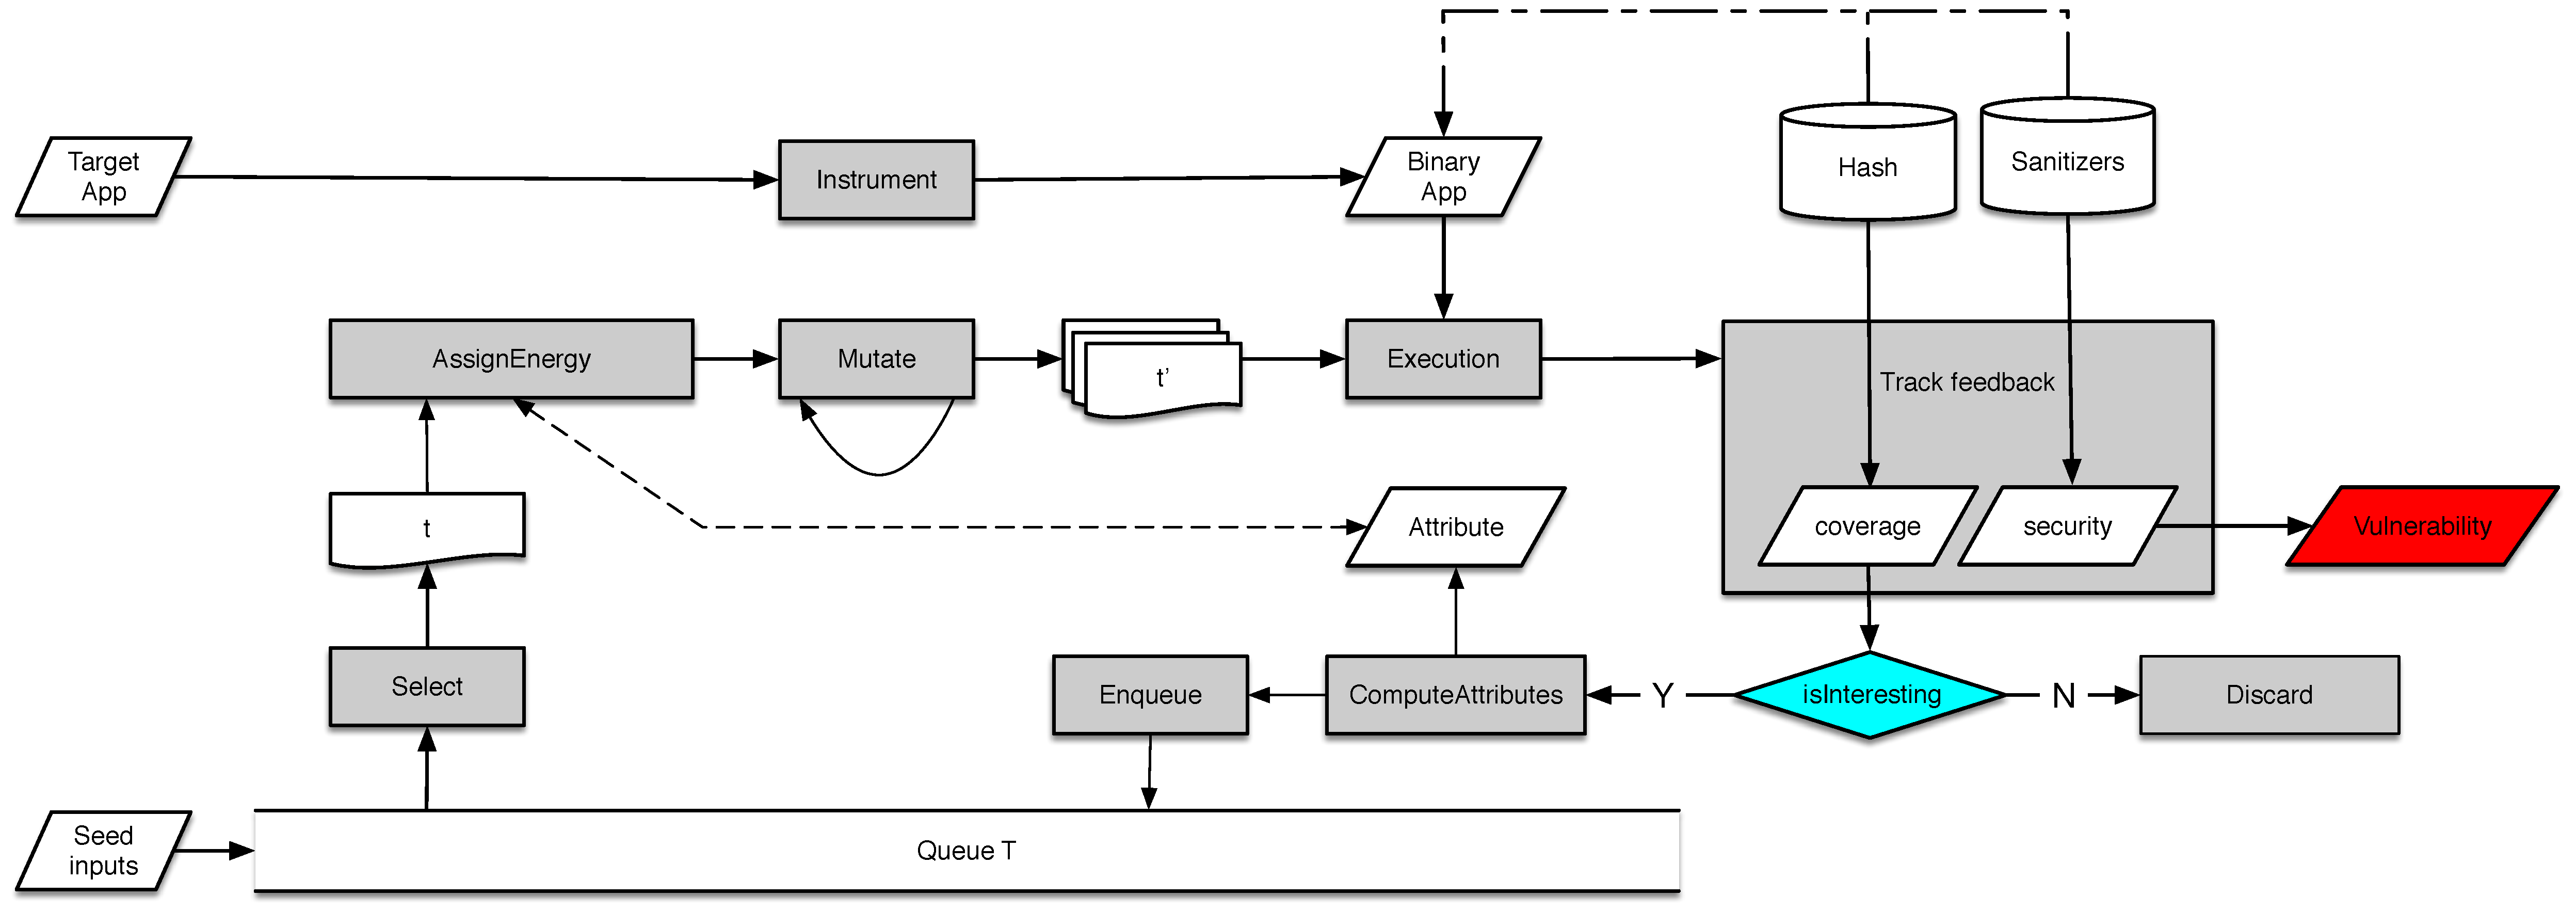
\includegraphics[width=6in]{pic/AFL.eps}
%    \caption{The general workflow of AFL  based greybox fuzzing}
%    \label{AFL}
%\end{figure*}


After instrumenting target program, AFL executes it with some initial seeds. Then, it maintains a queue of test cases and performs an evolutionary fuzzing loop as below:
\begin{enumerate}
\item \textbf{Selecting Seed:} select seed that worth fuzzing from testcase queue with a specific policy (e.g., according to execution time, seed length, and hit number); 
\item  \textbf{Assigning Energy:} calculate and assign energy for selected seed based on its attributes (e.g., execute time, bitmap size, etc.), where the energy of a seed represents number of new test cases that generated from the seed by mutation; 
\item  \textbf{Mutating Input:} mutate seeds using different kinds of mutation operators to generate a batch of new test cases;
\item  \textbf{Executing Target:} feed these new test cases to target application and execute them at a high speed as possible;
\item  \textbf{Tracking Feedback:} track run-time feedback including code coverage, security violation and so on. Meanwhile, vulnerabilities are reported if security violations are detected.
\item  \textbf{Filtering Testcase}: compute and update attributions of testcases, put those good testcases that contributing to code coverage into seed queue, and go to step 1).
\end{enumerate}


Following above continuous evolutionary loop, AFL could generate optimized seeds that explore new execution paths, and thus evolve towards a higher code coverage. As a result, the probability to trigger crashes is increased. The main concepts of AFL fuzzing is described in the following:
 
\subsection{Instrumentation} 

AFL's instrumentation captures basic block transitions, along with coarse branch-taken hit counts. A sketch of the code that shows in listing \ref{instrument} is injected at each branch point in the program. 

\begin{lstlisting}[ frame=single, label= instrument, basicstyle=\small, caption= AFL's Instrumentation]  
cur_location = <COMPILE_TIME_RANDOM>; 
shared_mem[cur_location ^ pre_locatiom] ++;
pre_location = cur_location >> 1;
\end{lstlisting}
The variable $cur\_location$ identifies current basic block. Its random identifier is generated at compile time. Variable $shared\_mem[]$ is a 64 KB shared memory region. Every byte that is set in the array marks a hit for a particular tuple  $(A, B)$ in the instrumented code, where basic block $B$ is executed after basic block $A$. The shift operation in Line 3 preserves the directionality [(A, B) vs. (B, A)]. A hash over $shared\_mem[]$ is used as path identifier. AFL uses coverage information to decide which generated input to retain for fuzzing. Also decides which input to be the priority choice and how long the input will be fuzzed. 
 
\begin{algorithm}[t]
\caption{AFL Greybox Fuzzing} 
\label{aflalgo}
\hspace*{\algorithmicindent} \textbf{Input}: seeds $S$, program $P$

\hspace*{\algorithmicindent} \textbf{Output}: crashes $Tx$
\begin{algorithmic}[1]
    \STATE $Queue \leftarrow S$ ;
    \WHILE{true} 
        \STATE $t \leftarrow$ \texttt{Select}($Queue$);
        \FOR{$i$  from $0$ to Length($t$)}
            \STATE $t' \leftarrow$ \texttt{DeterministicMutate}($t$, $i$);
            \STATE $runResult \leftarrow$ \texttt{RunProgram}($P$, $t'$);
            \IF{$runResult$ is crash}
                 \STATE \texttt{SaveCrashInfo}($runResult$, $Tx$);
            \ENDIF
    
            \IF{$runResult$ is Interesting}
                \STATE \texttt{AddToQueue}($t'$, $Queue$);
                \STATE \texttt{ComputeAttribute}($t'$);
            \ENDIF
        \ENDFOR    
        \STATE $energy \leftarrow$ \texttt{AssignEnergy}($t$);
        \FOR{$i$  from $0$ to $energy$}
            \STATE $t' \leftarrow$ \texttt{MutateInput}($t$, $i$);
            \STATE $runResult \leftarrow$ \texttt{RunProgram}($P$, $t'$);
            \IF{$runResult$ is crash}
                \STATE \texttt{SaveCrashInfo}($runResult$, $Tx$);
            \ENDIF
    
            \IF{$runResult$ is Interesting}
                \STATE \texttt{AddToQueue}($t'$, $Queue$);
                \STATE \texttt{ComputeAttribute}($t'$);
            \ENDIF
        \ENDFOR    
    \ENDWHILE
\end{algorithmic}
\end{algorithm}


Algorithm \ref{aflalgo} illustrates detailed fuzzing process through AFL's implementation. If AFL is provided with seeds $S$, they are added to the $Queue$. Otherwise, an empty file is generated as a starting point.

\subsection{Selecting Seed}
AFL determines a seed if it is $faverable$ based on its length and execution time. A seed will be marked as $favorable$ if it is the fastest and smallest input for any of the edges it exercises.  In process of selecting seed, these $favorable$ seeds will be selected with priority. Non-favorable seeds will be ignored with random probability.

\subsection{Assigning Energy}
The energy of a seed $t$ refers to number of new test cases that generated from $t$ after applying various mutation operators. In deterministic stage, AFL determines a seed's energy according to its length. And in havoc stage, AFL firstly determines the basis energy based on its execution time and average execution time. Then it updates total energy based on others attributes like block transition coverage(i.e., bitmap\_size), handicap, depth and so on.  

\subsection{Mutating Input}
In the act of mutating input, AFL utilizes some typical mutation operators to modify the initial seed, and generate a batch of new test cases. These mutation operators include Flips, Interesting, Arith, Extra and Splice in the following. In determined stage of mutation, these mutation operators will be used separately and sequentially to generate new test cases; And in havoc stage, AFL would mutate the seed by randomly choosing a sequence of mutation operators and apply them to random locations in the seed file. 

These mutation operators in AFL  are:
\begin{itemize}
\item  \textbf{Flips:} simple bitflip, two bitfilp, four bitflip, etc. 
\item  \textbf{Interesting:} set "interesting" bit, bytes, words, dwords.
\item  \textbf{Arith:} addition or subtraction of bytes, words or dwords.
\item  \textbf{Extra:} block deletion, block insert, overwrite, etc.
\item  \textbf{Splice:} splice two distinct input files at a random location.
\end{itemize}

\subsection{Tracking Feedback}
When a new test case is generated, it is fed to target program and executed by AFL. At run-time, feedback including code coverage and security violation are tracked.  AFL determines an input to be interesting only if that input has contribution to code coverage. Intuitively, AFL retains inputs that invoke a new block transition or a path where a block transition is executed twice while it normally executes only once. If the generated input $t^{'}$ crashes the program, it is added to a set of crashing inputs. A crash input that is also interesting will be marked as a unique crash. 

\subsection{Filtering Testcase}
If the generated input $t^{'}$ is considered to be interesting, AFL will run a calibration stage to compute and update its attributes, then add it into the queue. These attributes are  important because they are the basis for energy assignment. More specifically, these attributes include execution, bitmap, hit numbers and so on.

\section{New Insights}\label{newinsight}
During the process of using AFL based greybox fuzzers (e.g., AFL and AFLFast), we have some new insights about existing AFL's fuzzing energy distribution strategy. In this section, a detailed description of two insights is illustrated.

%\textbf{Insight 1: } Existing energy distribution strategies discriminate against time-consuming (TC) paths, which are usually paths containing long loops.  TC paths are ignored with large probability, and given little energy even if not ignored. At the select stage, AFL will prefer to choose the test case that execute faster and its size is smaller. And at the stage of compute the energy amount, the basis of the energy is determined by its execute time.  The core idea to determine the basis energy is the longer execute time, the smaller energy assigned, the maximize basis is 30 times of minimize basis. The detailed rules is shown in Table \ref{EnergyBasis}.
%\begin{table}[hbpt]
%\centering
%\label{EnergyBasis}
%\caption{Basis Energy Determine Rules}
%\begin{tabular}{|l|}
%\hline
%q $\rightarrow$ exec\_us * 0.10      $>$  avg\_exec\_us    $\rightarrow$  perf\_score = 10; \\
%q $\rightarrow$ exec\_us * 0.25      $>$  avg\_exec\_us    $\rightarrow$  perf\_score = 25;\\
%q $\rightarrow$ exec\_us * 0.50      $>$  avg\_exec\_us    $\rightarrow$  perf\_score = 50;\\
%q $\rightarrow$ exec\_us * 0.75      $>$  avg\_exec\_us    $\rightarrow$  perf\_score = 75;\\
%q $\rightarrow$ exec\_us * 2.00      $<$  avg\_exec\_us    $\rightarrow$  perf\_score = 150;\\
%q $\rightarrow$ exec\_us * 3.00      $<$  avg\_exec\_us    $\rightarrow$  perf\_score = 200;\\
%q $\rightarrow$ exec\_us * 4.00      $<$  avg\_exec\_us    $\rightarrow$  perf\_score = 300;\\
%\hline
%\end{tabular}
%\end{table}
%
%Where the $exec\_us$ represent the execute time of the test case $q$, and the $avg\_exec\_us$ represent the average execute time. $perf\_score$ is the score used for assigning energy.
%
%For institution, take following code fragment listed in the Listing \ref{TCPath} as an example to illustrate the discrimination against time-consuming paths. Considering the two paths distinguished by buf[0], there are two same crash bugs (i.e. crash A, crash B)  at the end of each path. The existing AFL's energy distribution  strategy is based on the execution time of the test case, the size of the bitmap and so on. Let the execute time of each instrument be one second. The total execute time of Path A to trigger crash A is 10002s, while the execute time of Path B to trigger crash B 14s, and the bitmap size of path A crash and path B crash is 3 and 7. Then based on the computation formula in AFL, the energy score of Path A maybe 7.5 (i.e. 10 $\times$ 0.75)  and the energy score of path B maybe 450 (i.e. 300$\times $1.5). That means that  the time-saving path (Path B)'s energy is 60 times larger then time-consuming path (Path A). 
%
%This discrimination makes it difficult to detect vulnerabilities buried in TC paths, such as crash A behind long loop. Furthermore, when the execute time is larger than the setting limit time of AFL, it may obtain hang, but never detect these kind of crashes.  Thus, energy assignment should give TC  paths opportunities and energy in order to balance the probabilities to detect bugs in time-consuming and time-saving paths.
%
%\begin{lstlisting}[float, language=C++,caption=Sample code contain Time-Consuming path, label=TCPath]
%#include "stdio.h"
%int main (int argc, char ** argv){
%    char buf[8];
%    if(read(0, buf, 8) < 1){
%        printf("Hum ?\n")
%        exit(1);
%    }
%    
%    if(buf[0] == 'a'){  //Path A
%        char * arr;
%        for(int i = 0; i< 10000; i++){
%               ......    
%        }
%        
%        if(buf[6]=='g' && buf[7]=='h' ){
%            abort();        // crash A
%        }
%    
%    }else if(buf[1]=='b'){   // Path B
%        if(buf[2] == 'c'){ 
%             printf("reach c\n");
%            if(buf[3]=='d'){ 
%                 printf("reach c\n");
%                if(buf[4]=='e'){
%                    printf("reach c\n");
%                    if(buf[5]=='f'){ 
%                        printf("reach c\n");
%                        if(buf[6]=='g' && buf[7]=='h'){  
%                            abort();        // crash B            
%                        }else printf("error\n");                        
%                    }else printf("error\n");                    
%                }else printf("error\n");            
%            }else printf("error\n");    
%        }else printf("error\n");    
%    }
%}
%\end{lstlisting}


\begin{figure}[t]
    \centering
    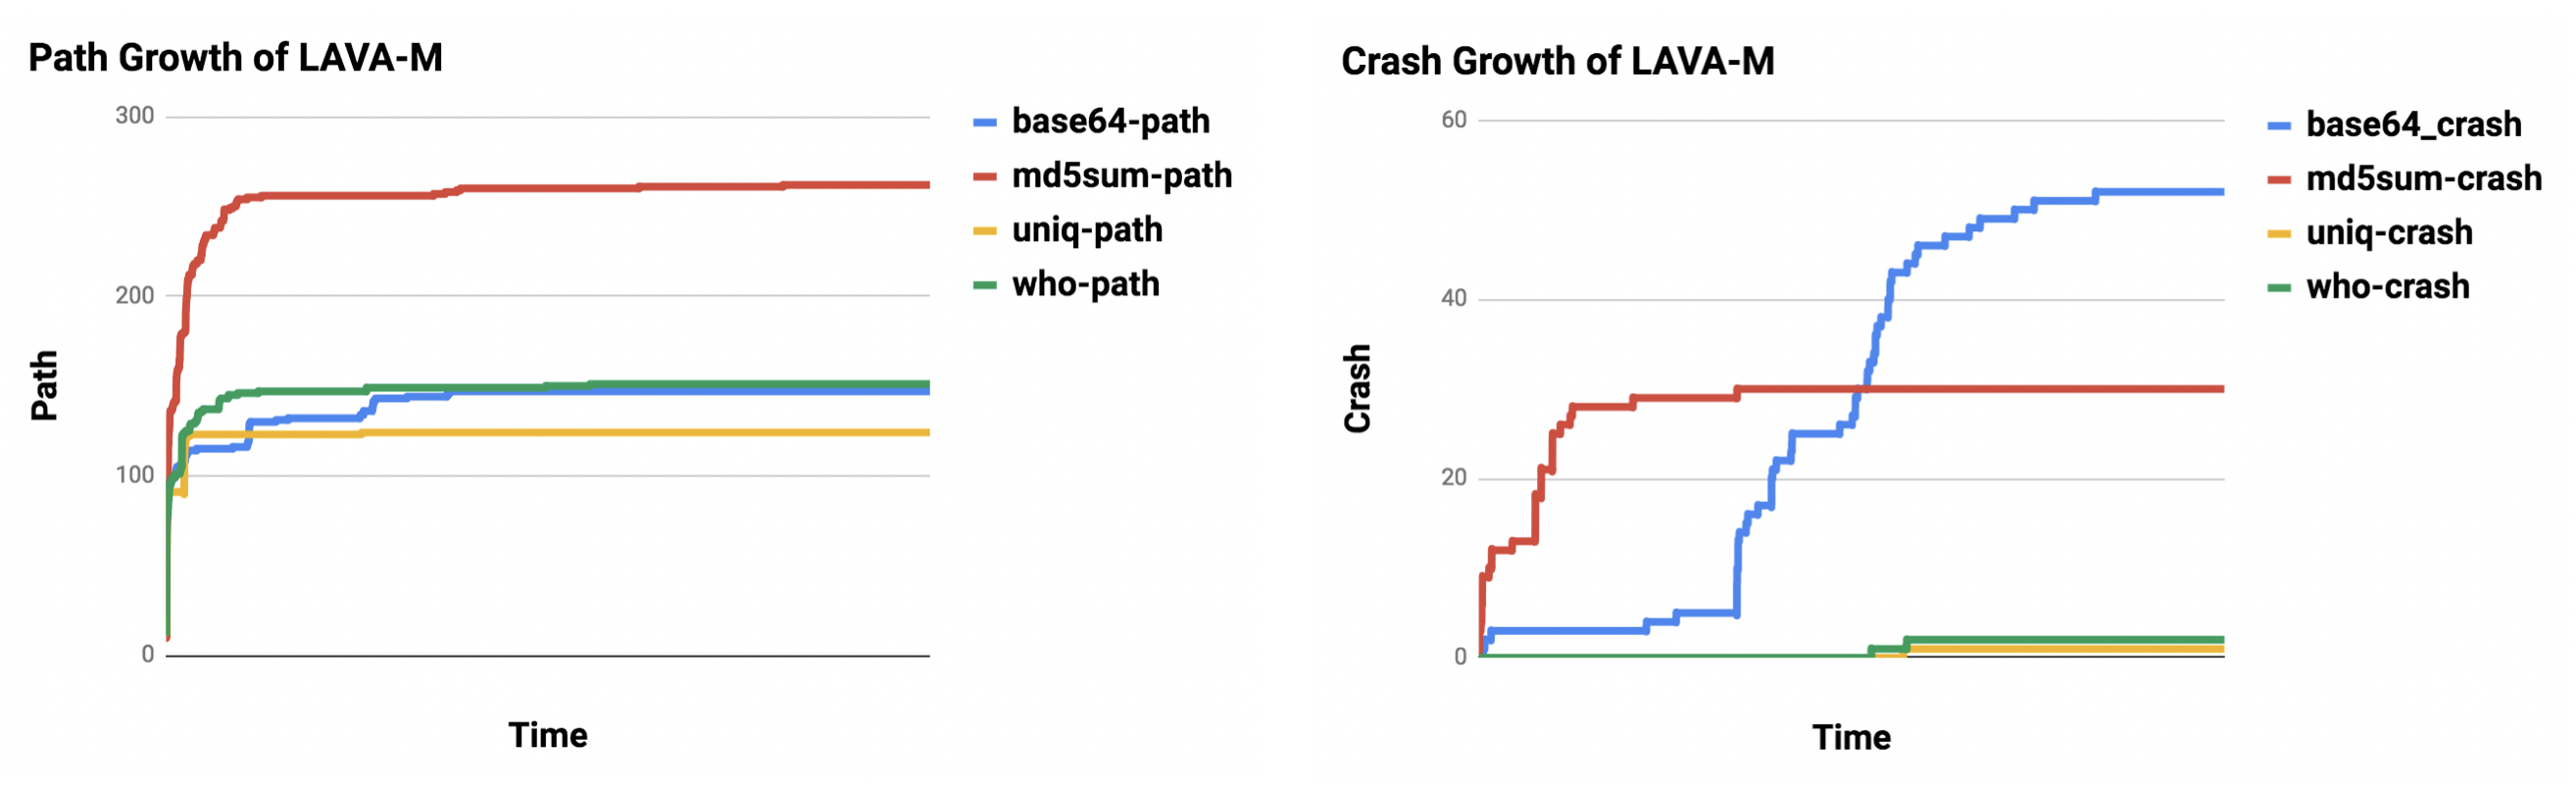
\includegraphics[width=3.5in]{pic/insight11.png}
    \caption{path and crash growth over time}
    \label{path-crash-growth}
\end{figure}
%explain your experimental setup?
%\gl{check the legend on the right: base64})

\textbf{Insight 1: } Growth of paths follows the same pattern, while growth of crashes has no definite rules. The Fig.\ref{path-crash-growth} is a statistical result of path growth and crash growth of LAVA-M \cite{lava} benchamrk fuzzed by AFL. As shown in Fig.\ref{path-crash-growth}, number of total path increases quickly at the beginning, and growth rate gradually becomes flat over time. Finally, it will become harder to find new path. And slop of growth curve is approximating zero. A natural reason is that discovery of new path is a Coupon Collector’s Problem (CCP) \cite{ferrante2014coupon}. After finding $i-1$ new paths, the probability of finding the $i$th new path is $P_{i}= (N-i+1)/N$, where $N$ is the number of total paths. From this formula, we can see that the discovery of new paths is increasingly difficult over time. Compared with path growth pattern, occurrence and increment of crashes are completely different. There is no universal model for the emergence and growth of crashes. As can be seen from above Fig. \ref{path-crash-growth}, crash may appear very early. It also may occur very late. Crash may grow faster at the beginning and then not grow later. It also may not grow at first, and then grow faster later. The reason behind this phenomenon is that direct cause of crash discovery is not increment of path coverage, but whether regions where vulnerabilities resided are explored. 

%
%\begin{lstlisting}[float, language=C++,caption=Sample code of energy distribution, label=DirectPath]
%#include "stdio.h"
%int fun (const uint8_t *Data, size_t Size, bool e){
%   if(e = true && Size ==22){                  // Path A
%      uint64_t x = 0;
%      int64_t  y = 0;
%      int32_t z = 0;
%      uint16_t a = 0;
%      memcpy(&x, Data, 8);  
%      memcpy(&y, Data + 8, 8);  
%      memcpy(&z, Data + 16, sizeof(z));  
%      memcpy(&a, Data + 20, sizeof(a));  
%     
%      if(x = 10 && y == 0xbaddcafedeadbeefUL)
%             abort();       
%       
%  }else if (e == false && Size < 22){    // Path B
%     printf("%d\n", *Data);
%      uint64_t x = 0;
%      memcpy(&x, Data, 8);  
%      if(x>10)
%          abort();
%  }
%}
%\end{lstlisting}

If those regions that are more likely for a vulnerability to reside are prioritized and strengthened to fuzz, related vulnerabilities buried in these regions will be detected faster. Furthermore, more bugs could be found during the same period of time. 

There are some common intuitions that sensitive region(i.e. region containing much memory or string related operators), complex region, deep region, and rare-reach region are more likely to be vulnerable due to developer negligence and inadequate testing. Thus, guide fuzzing toward these promising vulnerable regions and spend more fuzzing energy on them will improve the efficiency of fuzzing tool. 
%\gl{why is sensitive region prone to vulnerabilities? The rest are institutive, not sensitive region.}


%For the institution, take the following code fragment listed in the Listing \ref{DirectPath} as an example to show the rationality of promising area deserve more energy. Considering the path A and path B in Listing \ref{DirectPath}, path A contains more sensitive instruments like memcpy(). Also, it is more complicated than path B for it contains more instruments, and the bug is located deeper and rare-to-reach. Then we should spend more energy on Path A, no matter if there are bugs or not.
%
%Thus,  directed fuzzer prioritize fuzzing these vulnerability-promising areas and spend more fuzzing energy on these areas will improve the efficiency to detect vulnerabilities. 


\textbf{Insight 2: } Existing energy distribution strategy only considers calculation of mutations numbers. It does not consider scheduling of distribution ratio of different kinds of mutation operators. The energy refers to the number of new test cases generated by mutating seed using various granularity mutation operators. It is calculated based on seed's attributes such as execution time, bitmap size, depth, hit numbers and so on. However, scheduling of distribution proportion for different kinds of mutation operations in assigned number does not get enough attention it deserves. In determined stage of mutation, AFL applies mutation operators (e.g., Flips, Interesting, Arith, Extra, and Splice) separately and sequentially to generate new test case; And in havoc stage, AFL would mutate the seed by randomly choosing a sequence of different mutation operators and apply them to random locations in the seed files. 

\begin{figure}[t]
    \centering
    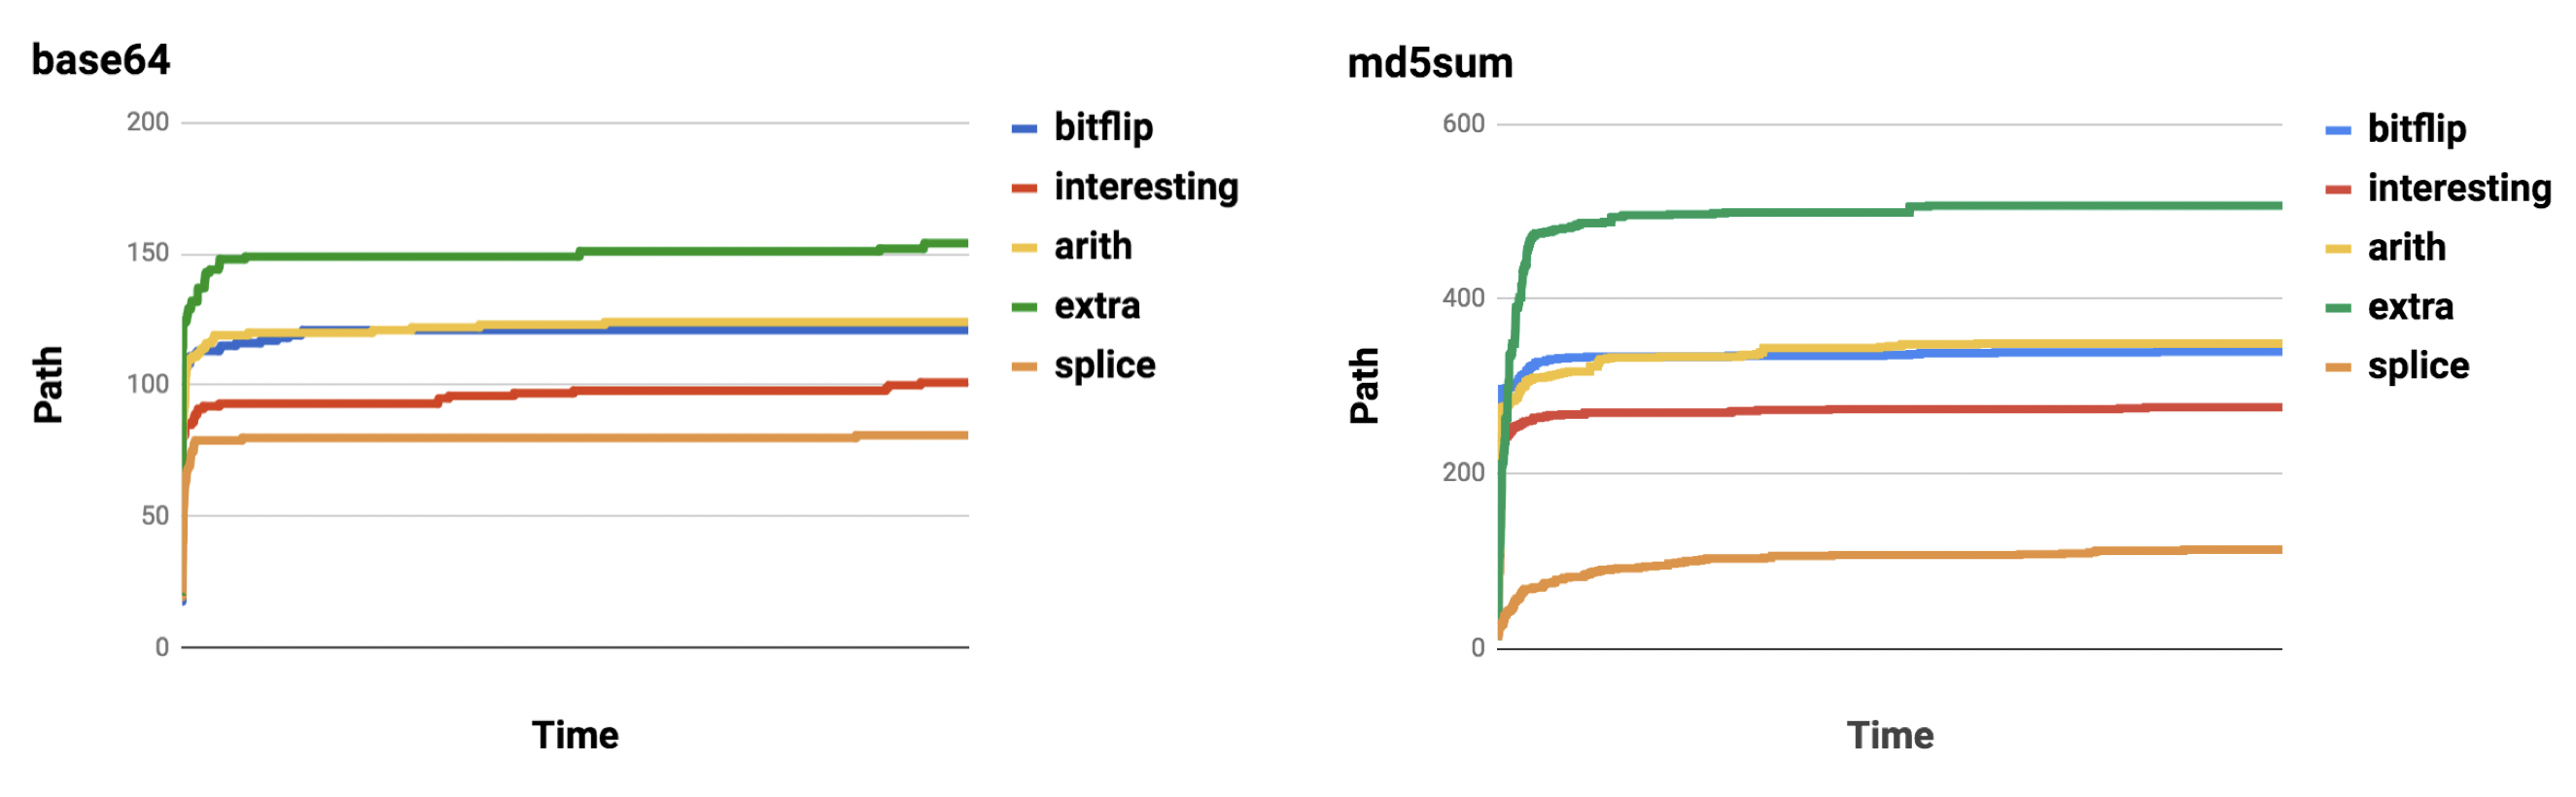
\includegraphics[width=3.5in]{pic/insight22.png}
    \caption{path growth using different mutators }
    \label{FineCoarseEffect}
\end{figure}

Experimental evaluation of each kind of mutation operators are performed on LAVA-M \cite{lava}, and the results are listed in Fig. \ref{FineCoarseEffect}. It indicates that different mutators have different abilities to trigger new path. Extra mutations have better ability to generate diversity test case, which is more helpful to the path growth. On the other hand, splice mutators perform poor. (2) The effect of combining multiple kinds of mutators is better than the effect of using single kind of mutator.% (3) The coarse-grained mutators are better than fine-grained mutators on helping path growth. 
However,  randomly choosing mutators without scheduling may cause overuse of some low effective mutation operators, and lack of diversity.


Thus, the energy distribution should consider not only the number of mutations but also the proportion of different kinds of mutation operators in assigned number. Despite the fact that finding new path will become more and more difficult, the proportion of mutation operations who has better ability to trigger new paths should gradually increase over time.


 

